\selectlanguage{spanish}
\section*{Introducción}

En este artículo continuaremos viendo más operativa y funciones de
Octave que podemos usar con polinomios. Además vamos a explicar las
instrucciones más usadas para programar: el comando \textit{if}, el
comando \textit{while} y el comando \textit{for}. Con estos comandos ya
somos capaces de realizar programas y funciones muy sofisticados. En
el próximo número os hablaremos de unos comandos más específicos como
son el \textit{do-until} y \textit{switch}. Finalmente un reto se os
dejará pendiente para que os divirtáis, pongáis en práctica lo
aprendido y tengáis la posibilidad de ganar un obsequio.

\section{Comandos: \textit{if}, \textit{while} y \textit{for}}

Cuando ejecutamos un programa, en términos muy básicos y generales,
seguimos un orden específico en la ejecución. En general este orden es
el de la aparición del programa. En esta secuenciación nos podemos
encontrar con: variables, expresiones, otras funciones, una selección,
una iteración, etc. En definitiva, una secuencia de flujo de
eventos. Los eventos a los que vamos a prestar atención en este número
son los eventos de selección mediante el comando \textit{if} y los de
iteración mediante los comandos \textit{while} y \textit{for}.

\subsection{Comado \textit{if}}
Este comando es el que permite a Octave tomar decisiones. Tenemos tres
formatos para poder usar el comando \textit{if} que mostramos en el
Cuadro \ref{tab:if}.
\begin{table}[!ht] 
\begin{mybox}%{c}{\textwidth} 
%\begin{table}  
\begin{tabular}{l|l|l}
    \begin{minipage}{0.3\linewidth}
\begin{verbatim} 
if (condition) 
  then-body
endif
\end{verbatim}
\end{minipage}&
    \begin{minipage}{0.3\linewidth}
\begin{verbatim} 
if (condition)
  then-body
else
  else-body
endif
\end{verbatim}    
    \end{minipage}&
    \begin{minipage}{0.3\linewidth}
\begin{verbatim} 
if (condition)
  then-body
elseif (condition)
  elseif-body
else
  else-body
endif
\end{verbatim}    
\end{minipage}\\
 \end{tabular}
%\end{table}
\end{mybox}\caption{Tres maneras de usar el comando \textit{if}}\label{tab:if}
\end{table}

Veamos unos ejemplos de funciones que muestren el potencial del
comando \textit{if}. El primer ejemplo calcula si un número es par o
impar y el segundo dados tres números calcula el máximo de
ellos. Cópialos y ejecútalos en tu ordenador y podrás entender su
mecanismo. Recuerda que cuando grabamos funciones en archivos de
Octave, estas deben grabarse con el mismo nombre y con extensión
\emph{.m}. Es decir la primera función la grabarás como
\emph{paridad.m} y la segunda como \emph{maximo3.m}.

\begin{center}\textbf{Ejemplo 1}\end{center}
\begin{octavebox}
\begin{verbatim}
function paridad(x)
  if (rem (x, 2) == 0)
    printf ("x es un número par\n");
  else
    printf ("x es un número impar\n");
endif
endfunction
\end{verbatim}
\end{octavebox}

\begin{center}\textbf{Ejemplo 2}\end{center}
\begin{octavebox}
  \begin{verbatim}
function max=maximo3(a,b,c)
  if (a>b && a>c)
    max=a;printf ("x es un número par\n");
 elseif (b>a && b>c)
   max=b;
 else
   max=c;
endif
endfunction
\end{verbatim}
\end{octavebox}

Si has ejecutado estas dos funciones han aparecido las funciones
implícitas de Octave siguientes:
\begin{itemize}
\item \textit{rem(x,y)}: calcula el resto de dividir $x$ entre $y$.
\item \textit{printf('Texto')}: imprime por pantalla al usuario el mensaje Texto.
\item \textit{\textbackslash n}: realiza un salto de línea.
\end{itemize}

\subsection{Comado \textit{while}}

En programación un bucle es una parte de programa que puede ser
repetida varias veces mientras se cumpla cierta condición. También
podría no ser ejecutado si la condición no se diera. En Octave el
comando más simple de realizar un bucle es \textit{while}. Podemos ver
su notación como sigue:

\begin{mybox}
     \begin{verbatim} 
while (condition)
  body
endwhile
\end{verbatim}
\end{mybox}

Lo primero que realiza el comando \textit{while} es el chequeo de la
condición \emph{condition}. El resultado de este chequeo es un valor
booleano: si es cierto se ejecutarán las instrucciones incluidas en el
\emph{body}. De nuevo se chequeará la condición \emph{condition} y si
vuelve a ser cierta se ejecutará de nuevo el \emph{body}. Y así, hasta
que la condición no se cumpla y se salga del bucle \textit{while}. En
el caso en que la condición \emph{condition} sea un vector o una
matriz ésta será cierta si no es vacía y todos los elementos son no
cero.

Veamos un ejemplo de un programa que, dado un número que es potencia de dos, nos comunica cuál es esa potencia.
\begin{octavebox}

\begin{verbatim}
function potencia=potencia2(n)
potencia=0;
while (rem(n,2)==0 && n>0)
  n=n/2 ; 
  potencia=potencia+1; % esto puede hacerse también como potencia++
end
\end{verbatim}
\end{octavebox}

Este programa puede ser optimizado, ya que si introduces un número que
no es potencia de 2 te da una respuesta errónea puesto que el programa
se ejecuta con la premisa de que la entrada o input es una potencia de
2. ¿Cómo harías un programa que no tiene en cuenta esa premisa? Te
ofrecemos una solución con la siguiente función:

\begin{octavebox}
\begin{verbatim}
% Suponemos n es un número natural

function potencia=potencia2_mejorado(n)
potencia1=0;

if (n<0)
  disp('El número debe ser un número natural')
  break
end

if (n==0)
  disp('El 0 no es potencia de 2')
  break
end

while (n>1)
    if (rem(n,2)==0)
      n=n/2 ; 
      potencia1=potencia1+1; % esto puede hacerse también como potencia++
    else
      disp('El número no es una potencia de dos. ¿Me querías engañar? ;>')
      break
     endif
endwhile
	  
if (n==1)
  potencia=potencia1;
end
\end{verbatim}
\end{octavebox}

Esta solución se deja unos pocos casos sin solucionar, ¿los has detectado?. Observa el comando \textit{break}, es una sentencia que puede encontrarse dentro de un bucle y que cuando se ejecuta sale del bucle directamente. 

\subsection{Comado \textit{for}}

El comando \textit{for} se usa para realizar bucles. La sintaxis es la
siguiente:
\begin{mybox}
\begin{verbatim} 
for var = expression
  body
endfor
\end{verbatim}
\end{mybox}

Te exponemos a continuación, varios ejemplos de cómo puede ser usado
el comando \textit{for} con los que esperamos puedas entender su
mecanismo.

\begin{enumerate}
\item Siendo la variable \emph{var} un contador:
\begin{octavebox}
  \begin{verbatim}
%Vamos a calcular el factorial de n
function fact=factorial(n)
fact=1;
for i=2:n
   fact=fact*i;
end
\end{verbatim}
\end{octavebox}
\item Siendo \emph{expression} una matriz:
\begin{octavebox}
  \begin{verbatim}
for i=[1 2;3 4;5 6]
  i
endfor
\end{verbatim}
\end{octavebox}
Como observarás recorriendo el código de esta forma recorre las
columnas de la matriz.
\item Siendo la variable \emph{var} un contador de una frase:
\begin{octavebox}
  \begin{verbatim}
contrafrase=[];
frase=["Adolfo es un chico que vive lejos de aqui"]
for i=length(frase):-1:1
    frase(i)
    contrafrase=[contrafrase,frase(i)];
end
contrafrase
\end{verbatim}
\end{octavebox}
\end{enumerate}
\section{El reto del número anterior}
En el número anterior os dejamos en la Sección 2 un desafío: un
programa que dados cuatro puntos cualesquiera del plano calcule el
polinomio de grado 3 que pasa por ellos y que realice un dibujo donde
representa tantos los puntos dados como el polinomio calculado. El
mejor programa que nos ha llegado es de \emph{João Viana López} a quien le
damos las gracias por seguirnos y aquí os dejamos su programa ganador.
\begin{octavebox}
  \begin{verbatim}
% Esta función calcula el polinomio cúbico que pasa por los puntos
% (a1,b1), (a2,b2), (a3,b3) y (a4,b4)
% x es un vector con cuatro componentes, x=[a1 a2 a3 a4]              
% y es un vector con las correspondientes componentes compañeras, y=[b1 b2 b3 b4]   
 
function pol= polcubico(x,y)                                          % Lin 1
pol=vander(x)\y';                                                     % Lin 2
s=sort(x);                                                            % Lin 3
z=s(1)-2:0.5:s(4)+2;                                                  % Lin 4
zy=polyval(pol,z);                                                    % Lin 5
grid                                                                  % Lin 6
hold on;                                                              % Lin 7                                                                      
plot(x,y,'hr','markersize',15);                                       % Lin 8
plot(z,zy,'linewidth',2);                                             % Lin 9
hold off;                                                             % Lin 10
print('polinomios3','-color','-deps')                                 % Lin 11
\end{verbatim}
\end{octavebox}

Veamos el planteamiento que se ha realizado para llegar a esta
solución. Buscamos un polinomio $p(x)$ de grado tres que puede
escribirse como
\begin{equation}\label{eq:pol3}
p(x)=c_3 x^3+c_2 x^2 + c_1 x+ c_0.
\end{equation}
Lo que buscamos conocer son los coeficientes reales $c_3,c_2,c_1$ y
$c_0$; estas son nuestras incógnitas y el vector $[c_3\, c_2\, c_1\,
c_0]$ representa en Octave el polinomio que buscamos. De partida,
tenemos que los puntos dados $(a_1,b_1)$, $(a_2,b_2)$, $(a_3,b_3)$ y
$(a_4,b_4)$, constituyen el \emph{input} del programa a
desarrollar. Estos son puntos del polinomio y por tanto deben
satisfacer la ecuación (\ref{eq:pol3}). De esta manera obtenemos las
siguientes identidades:
\begin{equation}
\begin{array}{l}
c_0+c_1 a_1+c_2a_1^2+c_3a_1^3=b_1\\
c_0+c_1a_2+c_2a_2^2+c_3a_2^3=b_2\\
c_0+c_1a_3+c_2a_3^2+c_3a_3^3=b_3\\
c_0+c_1a_4+c_2a_4^2+c_3a_4^3=b_4\\
\end{array}.
\end{equation}
Recordando que las incógnitas son $c_3,c_2,c_1$ y $c_0$, las
ecuaciones anteriores pueden escribirse matricialmente como sigue:
\begin{equation}\label{eq:solsistema}
\left[
\begin{array}{cccc}
1 & a_1 & a_1^2 & a_1^3\\
 1 & a_2 & a_2^2 & a_2^3 \\
 1 & a_3 & a_3^2 & a_3^3 \\
 1 & a_4 & a_4^2 & a_4^3 \\
\end{array}\right] \cdot
\left[
\begin{array}{c}
c_0 \\
c_1 \\
c_2 \\
c_3 \\
\end{array}\right]=
\left[
\begin{array}{c}
b_1 \\
b_2 \\
b_3 \\
b_4 \\
\end{array}\right].
\end{equation}

La resolución del sistema matricial de la ecuación \ref{eq:solsistema}
nos da los coeficientes del polinomio buscado.  La matriz de
coeficientes de este sistema es un tipo particular de matriz (que
además vimos en el segundo número de este minicurso de Octave) y son
llamadas matrices de Vandermonde que se forman con el comando
\emph{vander} de Octave. ¿Cómo se resuelven los sistemas de ecuaciones
lineales en Octave? Con el comando \emph{\textbackslash}. Esto es
$A\textbackslash b$ donde $A$ es la matriz de coeficientes y $b$ el
término independiente del sistema. Con esta explicación es mucho más
fácil entender el programa expuesto como solución al reto que os
propusimos en el número anterior. ¡Espero que lo hayas disfrutado!

\section{Más sobre polinomios}
En el anterior artículo hablamos de como se trabajan los polinomios en
Octave, como se calculan sus raíces, como se multiplican, dividen,
suman y restan dos polinomios y como construir un polinomio mónico
dadas sus raíces entre otros. En este número vamos a ver funciones de
Octave más sofisticadas y que en proyectos más serios te pueden ser de
gran utilidad: el cálculo del máximo común divisor, la derivada e
integral de un polinomio y por último interpolación mediante splines.
\subsection{El máximo común divisor de dos polinomios}

Como recordarás el máximo común divisor (great common divisor,
abreviado en inglés g.c.d.) de dos números enteros es el mayor de los
divisores comunes. Así el 4 es el g.c.d. de 8 y 12. De manera similar
se puede definir el máximo común divisor de dos polinomios: es el
polinomio de mayor grado que divide a ambos polinomios. Octave puede
calcular el g.c.d de dos polinomios con el comando
\emph{gcd(p1,p2,...)}. Por ejemplo si tenemos el polinomio
$p(x)=x^3-10x^2+31x-30=(x-2)(x-3)(x-5)$ y
$q(x)=x^4-10x^3+32x^2-38x+15=(x-1)^2(x-3)(x-5$ claramente el polinomio
máximo común divisor es $(x-3)(x-5)$. Veamoslo en Octave:
\begin{octavebox}
\begin{verbatim}
octave:8> p1=poly([2 3 5])
p1 =

    1  -10   31  -30

octave:9> p2=poly([1 1 3 5])
p2 =

    1  -10   32  -38   15

octave:10> polygcd(p1,p2)
ans =

    1   -8   15
\end{verbatim}
\end{octavebox}

\subsection{Derivadas e integrales de polinomios}
La derivada e integral de un polinomio es calculada con Octave con los
comandos \emph{polyder(p)} y \emph{polyint(p)}. Por ejemplo, la
derivada del polinomio $4x^3+9x+3$ es el polinomio $12x^2+9$, y su
integral (tomando como constante de integración igual a 0) es
$x^4+\frac{9}{2}x^2+3x$. Veámoslo:
\begin{octavebox}
\begin{verbatim}
octave:1> p=[4 0 9 3];
octave:2> polyder(p)
ans =

   12    0    9

octave:3> polyint(p,0)
ans =

   1.00000   0.00000   4.50000   3.00000   0.00000

\end{verbatim}
\end{octavebox}

\subsection{Splines}
En bastantes aplicaciones de la ciencia y la ingeniería se tiene
conocimiento muy ajustado y parcial de un determinado
fenómeno. Ampliar información de este fenómeno de una manera más
global aun que no sea real pero si aproximada permite realizar serios
estudios de estos fenómenos. La interpolación es uno de los tantos
métodos que nos permiten realizar esto. Imaginemos por ejemplo, que
queremos determinar matemáticamente el perfil de una montaña y por
coste, sólo tenemos una cantidad limitada de puntos. Con esos puntos
buscamos aproximar el perfir real. Usando interpolación lo que se hará
es construir funciones simples de ser evaluadas que pasan por los
puntos conocidos(información parcial) y cuyo resultado no sea lejos de
la realidad. En general las funciones que usaremos deben ser fáciles
de evaluar y con buenas propiedades y quien mejor que nuestros amigos
\emph{los polinomios}. En este caso se habla de interpolación
polinómica.

Definimos una spline como una curva diferenciable definida a trozos
mediante polinomios. En Octave tenemos la función \emph{spline(X,Y)}
que calcula las splines que pasan por los puntos que determinal los
pares $(X,Y)$. Por defecto el commando $spline(X,Y)$ usa polinomios
cúbicos. Te animamos a que ejecutes el siguiente script para entender
su funcionamiento y ser capaz de realizar el reto que dejamos para
esta semana:
\begin{octavebox}
\begin{verbatim}
% Ejecutar este script para ver funcionamiento de spline
% 
% Sea una función conocida (en general esto no se conoce)
% f(x)=sin(x)+cos(2*x) 

% estos serían mis datos 
 X=-pi:0.4:2*pi;
 Y=sin(X)+cos(2*X);

% Calculamos la aproximación mediante splines de Octave

 aprox1=spline(X,Y)


% Vamos a comparar lo calculado con la función que en este caso es conocido 
% recuerda que normalmente no se conoce,
% sino no tendría sentido aproximar algo conocido
figure

% dibujamos la de verdad pero en una maya más densa para acercarnos a la función real
 Xd=-pi:0.05:2*pi;
 Yd=sin(Xd)+cos(2*Xd);
 plot(Xd,Yd,'b')
 hold on

% dibujamos la calculada

  plot(X,ppval(aprox1,X),'r')

legend ({"función conocida f(x)=\sin(x)+\cos(2x)", "aproximación mediante spline"})

  hold off
\end{verbatim}
\end{octavebox}

Investiga por tu propia cuenta el comando \emph{splinefit} y con ello intentes resolver el siguiente reto. Sé el primero en resolverlo.

%\begin{wrapfigure}{r}{\textwidth} 
\begin{mybox}
   \centering {\fontsize{20}{10}\selectfont\color{red} El Reto}
  %\begin{tabular}{cc}
  %  \begin{minipage}{0.2\linewidth}
  %    {\fontsize{10}{5}\selectfont\color{red} El Reto}
  %  \end{minipage}&
  %  \begin{minipage}{0.8\linewidth}
  %     \begin{figurebox}

   \begin{center}\scalebox{0.64}{% Title: glps_renderer figure
% Creator: GL2PS 1.3.8, (C) 1999-2012 C. Geuzaine
% For: Octave
% CreationDate: Wed May 28 10:45:39 2014
\setlength{\unitlength}{1pt}
\begin{picture}(0,0)
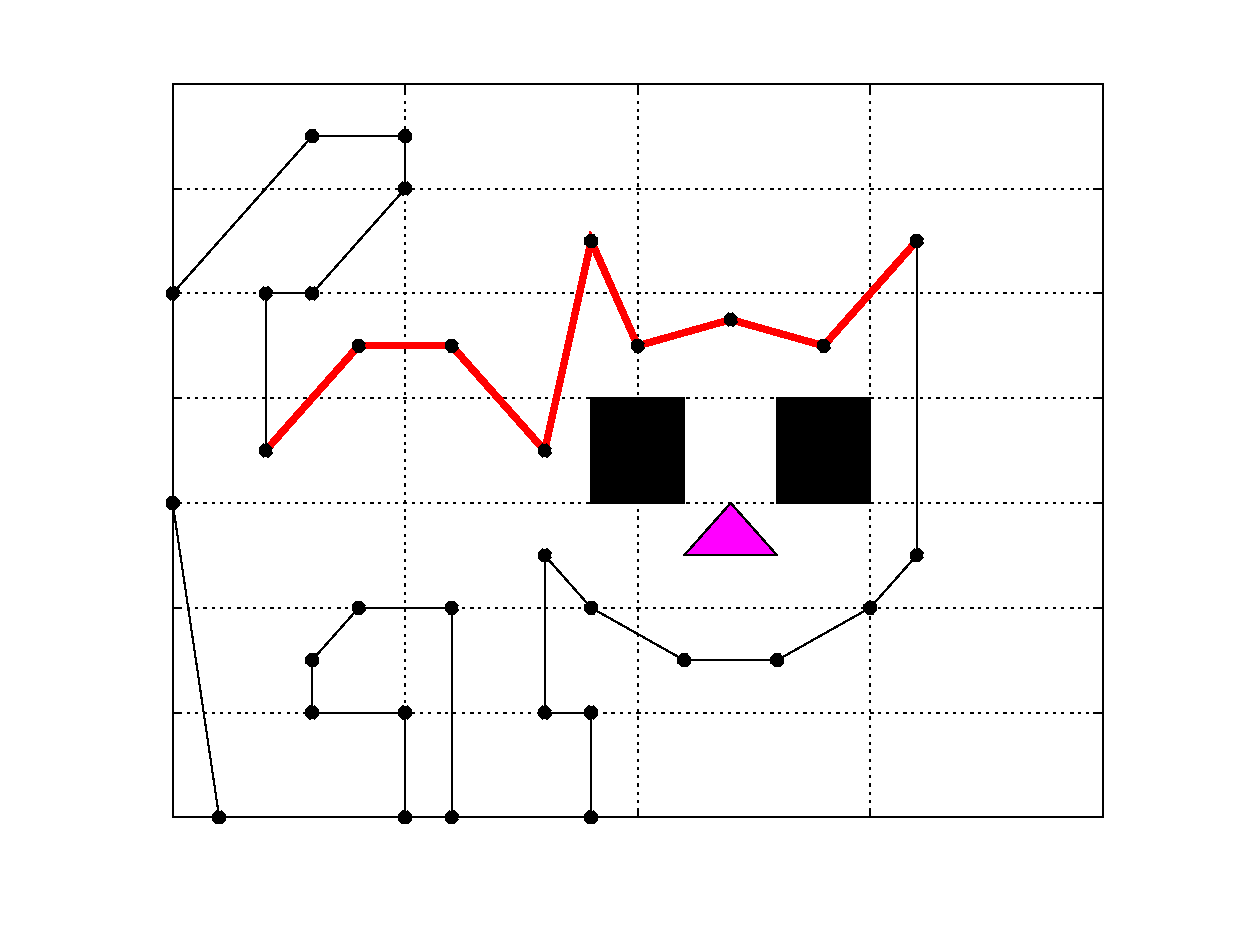
\includegraphics{gatito-inc}
\end{picture}%
\begin{picture}(576,432)(0,0)
\fontsize{10}{0}
\selectfont\put(74.88,42.5189){\makebox(0,0)[t]{\textcolor[rgb]{0,0,0}{{0}}}}
\fontsize{10}{0}
\selectfont\put(186.48,42.5189){\makebox(0,0)[t]{\textcolor[rgb]{0,0,0}{{5}}}}
\fontsize{10}{0}
\selectfont\put(298.08,42.5189){\makebox(0,0)[t]{\textcolor[rgb]{0,0,0}{{10}}}}
\fontsize{10}{0}
\selectfont\put(409.68,42.5189){\makebox(0,0)[t]{\textcolor[rgb]{0,0,0}{{15}}}}
\fontsize{10}{0}
\selectfont\put(521.28,42.5189){\makebox(0,0)[t]{\textcolor[rgb]{0,0,0}{{20}}}}
\fontsize{10}{0}
\selectfont\put(69.8755,47.52){\makebox(0,0)[r]{\textcolor[rgb]{0,0,0}{{2}}}}
\fontsize{10}{0}
\selectfont\put(69.8755,97.8171){\makebox(0,0)[r]{\textcolor[rgb]{0,0,0}{{4}}}}
\fontsize{10}{0}
\selectfont\put(69.8755,148.114){\makebox(0,0)[r]{\textcolor[rgb]{0,0,0}{{6}}}}
\fontsize{10}{0}
\selectfont\put(69.8755,198.411){\makebox(0,0)[r]{\textcolor[rgb]{0,0,0}{{8}}}}
\fontsize{10}{0}
\selectfont\put(69.8755,248.709){\makebox(0,0)[r]{\textcolor[rgb]{0,0,0}{{10}}}}
\fontsize{10}{0}
\selectfont\put(69.8755,299.006){\makebox(0,0)[r]{\textcolor[rgb]{0,0,0}{{12}}}}
\fontsize{10}{0}
\selectfont\put(69.8755,349.303){\makebox(0,0)[r]{\textcolor[rgb]{0,0,0}{{14}}}}
\fontsize{10}{0}
\selectfont\put(69.8755,399.6){\makebox(0,0)[r]{\textcolor[rgb]{0,0,0}{{16}}}}
\fontsize{10}{0}
\selectfont\put(298.08,409.6){\makebox(0,0)[b]{\textcolor[rgb]{0,0,0}{{Gatito}}}}
\end{picture}
}\end{center}
  % \end{figurebox}
Interpola mediante splines el lomo (parte roja) del gato.
  %  \end{minipage}
  %\end{tabular}\\
  Envía la solución a: \url{revista@revistasolucoes.com}
%\includegraphics[scale=0.4]{topimage.jpg}\\
    
\end{mybox}
%\end{wrapfigure}

%\vspace{3cm}
%\noindent
%\includegraphics[width=\textwidth]{pubmm2.png}

\newpage
%%% Local Variables: 
%%% mode: latex
%%% TeX-master: "informaticaeningenieria"
%%% End: 



